%Preamble--------
\documentclass[a4paper, 12pt]{article}
%Package_List ------------
\usepackage{fancyhdr}
\usepackage[a4paper,left=30mm,right=30mm,top=15mm,bottom=22mm]{geometry}
\usepackage{float}
\usepackage{graphicx}
\usepackage{mathptmx}
\usepackage[nottoc, notlot, notlof]{tocbibind}
\usepackage{tabularx}
\usepackage{titlesec}
\usepackage{enumitem}
\usepackage{multicol}
\usepackage[backend=bibtex,style=ieee,sorting=none]{biblatex}
\addbibresource{ref.bib}

%End Package_List ----------
\titleformat*{\section}{\huge\bfseries}
\titleformat*{\subsection}{\large\bfseries}
\titleformat*{\subsubsection}{\large\bfseries}
\titleformat*{\paragraph}{\normalsize\bfseries}
\titleformat*{\subparagraph}{\normalsize\bfseries}
\graphicspath{{./images/}}
\setlength{\headheight}{15pt}
\pagestyle{fancy}
\fancyhead{}
\fancyfoot{}
\setcounter{secnumdepth}{0}
\fancyhead[L]{\textbf{\leftmark}}
\fancyfoot[C]{\thepage}
\setlength{\parindent}{0ex}
\setlength{\parskip}{1.5em}
\linespread{1.3}
\title{Hindi Tweets Sentiment Analysis Using Transfer Learning}
%\subtitle{Abstract}
\author{Anubhav Mehra}
\date{\today}

%End Preamble -------------


\begin{document}
\begin{titlepage}
	\begin{center}
		\vspace*{1cm}
			\Huge{\textbf{Ph.D. Dissertation}}\\
			\Huge{\textbf{S.S.J University, Almora}}\\
			\vfill
			\line(1,0){400}\\[1mm]
			\large{\textbf{Hindi Tweets Sentiment Analysis Using Transfer Learning}}\\[3mm]
			\large{\textbf{Department Of Computer Science}}\\[1mm]
			\line(1,0){400}\\[1mm]
			By \textsc{Anubhav Mehra}
			
	\end{center}
\end{titlepage}
\begin{sloppypar}
\begin{center}
\textbf{ACKNOWLEDGMENT}
\end{center}
It is a genuine pleasure to express my deep sense of gratitude to my mentor and my Ph.D. supervisor Dr. Manoj Singh Bisht. His advice and approach have helped me to a very great extent to accomplish this task. 

I would also like to extend my gratitude to the Department of Computer Science, S.S.J University, Almora and all its faculty members who have been of great help during the course of this project.

Finally I would like to thanks my head Dr. Ashish Mehta, Department of Computer Science, DSB Campus Nainital for his immense help and providing me with time to complete my dissertation work.
\thispagestyle{empty}
\clearpage
\begin{center}
\textbf{DECLARATION}
\end{center}
I declare that this written submission represents my ideas in my own words and where others' ideas or words have been included, I have adequately cited and referenced the original sources. I also declare that I have adhered to all the principles of academic honesty and integrity and have not  misrepresented or fabricated or falsified any idea/data/fact/source in my submission. I understand that any violation of the above will be cause of disciplinary action by the University and can also evoke penal action from the sources which have thus not been properly cited or from whom proper permission has not been taken when needed.
\begin{flushright}
Anubhav Mehra \\
\today
\end{flushright}
\tableofcontents
\thispagestyle{empty}
\clearpage
\setcounter{page}{1}
\section{Introduction}
\begin{abstract}
\noindent Sentiment analysis is a \textbf{natural language processing} technique to find if the sentiment of the text is positive, neutral or negative. Traditionally, to train a model for sentiment analysis require very dense neural networks to train on very huge datasets. But, here we have used a technique called \textbf{Transfer Learning} that stores a model which has learned some knowledge, that we can leverage in solving some other tasks based on the knowledge of the previous model. Here we are using a language model called  \textbf{BERT(Bidirectional Encoder Representations from Transformers)}. BERT is a pertained model which learns using the learning techniques developed by Google. The BERT multilingual base model that we are using is pertained on the top 104 languages including Hindi. We then leverage the power of this model for the Sentiment analysis of the Hindi texts dataset that we've got. This allows us to achieve moderately high accuracy scores using a comparatively small dataset.
\end{abstract}

\subsection{Transfer Learning}
Transfer Learning is a Machine Learning method where a model that is trained for a certain task is utilized as the starting point for solving some other task i.e., to train a second model from the knowledge learned from the first model as well as the dataset. It is a very popular approach in natural language processing domain to solve problems such as getting the context of the text.

\begin{figure}[H]
\begin{center}
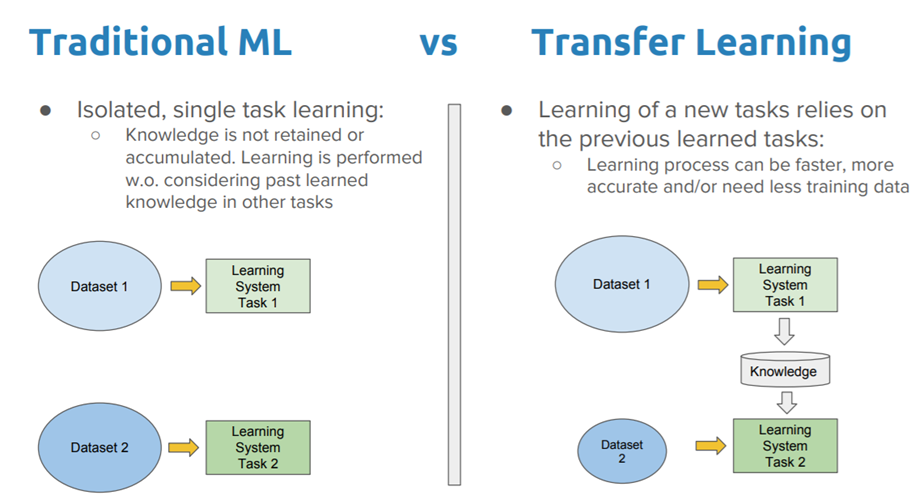
\includegraphics[scale=0.45]{tl.png}
\caption{Differentiation between Traditional and Transfer Learning Methodology. \label{tl}} %cite here guide to tl 
\end{center}
\end{figure}

The inspiration for transfer learning comes from us - humans, ourselves - where in, we have an inherent ability to not learn everything from scratch. We transfer and leverage our knowledge from what we have learn in the past for tackling a wide variety of tasks.\cite{sarkar_deep_2018}

\large \textbf{Deciding when to use Transfer Learning} \\ [0.5ex]
\normalsize
As with any technique at our disposal we must have a very clear reason on using transfer learning. First and foremost, we must realize that we can't use transfer learning in every situation. This is because for transfer learning to work we must have a model trained on a similar task. As with the problem concerned in our dissertation here, we have  a language model available which is trained in recognizing linguistic structure of  various languages. Now, we can leverage the power of this model to train a new model for our context analysis problem. If this is the case, you will realize that transfer learning is a very decent technique to use for acquiring better results and that too in very short amount of time than traditional methods. Now, with this out of the way you may want to use transfer learning if you have following conditions:
\begin{itemize}
\item{You have a smaller dataset}
\item{You are constrained on time}
\end{itemize}

\large \textbf{Applications of Transfer Learning} \\ [0.5ex]
\normalsize
There are various applications of Transfer Learning in variety of domains. In \textbf{Image Recognition}, transfer learning can be used to perform various imaging tasks. For e.g.,  a model trained to identify face can be used for facial recognition. Transfer Learning can also be used in \textbf{Speech Recognition} tasks.  For e.g., a model trained in a particular language for speech recognition can be used to train a model for speech authentication. But our key domain of interest where we are most interested in using this technique is \textbf{Natural Language Processing}. Transfer learning can be used to solve various tasks in  NLP. For e.g., a model trained in recognizing the linguistic structure of a language can be used to train a model to predict next word based on the series of words it gets in the previous sentences.

\subsection{Sentiment Analysis}
One such task in NLP is \textbf{Sentiment Analysis}. Sentiment Analysis or emotion AI, is the process in natural language processing  of subjective emotional analysis of the text. Primarily sentiment analysis finds if the emotional tone of a piece of writing is \textbf{\textit{positive, neutral or negative}}. \textbf{Table \ref{table: category}} lists some examples of what a sentiment analysis categorization may look like.
\begin{table}[H]
\caption{ Sentiment Analysis Categorization.\label{table: category}}

\begin{tabularx}{\columnwidth}{| X | X |}
\hline
Text & Category \\ [0.5ex]
\hline
\hline
That restaurant has a great food & Positive \\ [0.5ex]
\hline
He is my brother's colleague & Neutral \\ [0.5ex]
\hline
Bollywood movies are not entertaining & Negative \\ [0.5ex]
\hline
\end{tabularx}
\end{table}

As we can see it is easily understood by a human brain what sentiments these pieces of writing represent. But, for a computer this is a very challenging problem. It is a challenging problem because the way humans communicate using natural languages is extremely varied depending  upon \textit{subjectivity}, \textit{use of irony}, and the \textit{context} of the phrase. Not all verbs, nouns and pronouns can be treated equally when analyzing the emotional tone of the text. The tone of our phrases depends on how we are using them, when we are using them and for what we are using them. For e.g., the phrase \textit{absolutely everything}, can be an answer to a question like \textit{What are you so happy about?} or can equally be an answer to a completely opposite  question \textit{What are you so sad about?}. Thus, the emotional tone of the phrase can have completely separate meaning depending upon the various parameters. In the example above, the context of the phrase can alter the emotional meaning of the phrase completely. We'll see more about the challenges faced in Sentiment Analysis, in the following chapters.

\large \textbf{Applications of Sentiment Analysis} \\[0.5ex]
\normalsize
Listed below are some applications of Sentiment Analysis:
\begin{itemize}
\item{
\textbf{Social Media Monitoring: } Sentiment analysis is very useful tool to find out what is a general sentiment of people in social media towards a product, person, situation, trend or any such topic of interest.}
\item{
\textbf{Feedback Analysis: } Sentiment analysis can also be used to find the whether the  reception of new policies or workings of a company or of a government is positive or negative. This helps a company or government to evaluate their policies and performance using a well-defined metric.}
\item{
\textbf{Market Research: } Sentiment analysis can also be used to find what topics are viewed in positive and negative light in current landscape. This information can then be used to design or steer a companies marketing campaign to align with those sentiments.}
\end{itemize}


\begin{figure}[H]
\begin{center}
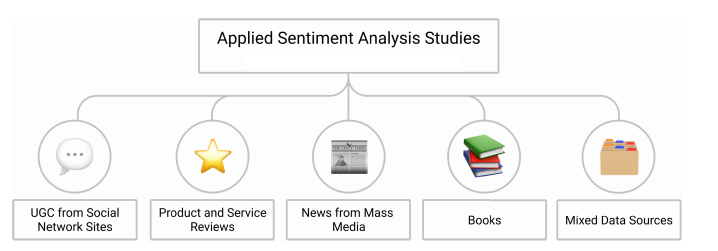
\includegraphics[scale=0.7]{cat.png}
\caption{Application of Sentiment Analysis. \label{cat}} %cite here the application of SA
\end{center}
\end{figure}

\subsection{Purpose}

The purpose of this project is to showcase the use of Transfer Learning in developing a model for Sentiment Analysis of Social Media Posts( tweets in this case) in Hindi Language. Thus, calculating the accuracy of the model trained on a relatively small dataset compared to those that would have been required if we would've followed a Traditional ML route. Hence, contributing in the field of Machine Learning and Data Science for any future project work in technology development.

\subsection{Dissertation Structure}
\textbf{Chapter 2:} This chapter discusses the literature review of this project. It discusses the concepts of this project, related an similar works done.

\textbf{Chapter 3:} This section describes the steps of the method followed to complete the project, which includes data sourcing, data preprocessing, model selection, model implementation, accuracy score calculation.

\textbf{Chapter 4:} This section describes the result and analysis of the project.

\textbf{Chapter 5:} The conclusion of the project is given in this section.

\textbf{Chapter 6:} This section contains the bibliography for this dissertation.
\clearpage

\section {Review of Literature}
\clearpage
\printbibliography
\clearpage

\end{sloppypar}
\end{document}
